%\documentclass[11pt,a4paper]{article}
\documentclass[11pt
  , a4paper
  , article
  , oneside
%  , twoside
%  , draft
]{memoir}

\usepackage{control}
\usepackage[numbers]{natbib}
\definecolor{babypink}{rgb}{0.96, 0.76, 0.76}
\definecolor{blizzardblue}{rgb}{0.67, 0.9, 0.93}

\begin{document}

\newcommand{\technumber}{
  RAON Control-Document Series\\
  Revision : v1.0,   Release : Nov. 04. 2015}
\title{\textbf{EPICS IOC on Raspberry Pi with MightyOhm Geiger Counter Kit}}

\author{박미정\thanks{mijoy0909@ibs.re.kr} \\

  Rare Isotope Science Project\\
  Institute for Basic Science, Daejeon, South Korea
}
\date{\today}

\renewcommand{\maketitlehooka}{\begin{flushright}\textsf{\technumber}\end{flushright}}
%\renewcommand{\maketitlehookb}{\centering\textsf{\subtitle}}
%\renewcommand{\maketitlehookc}{C}
%\renewcommand{\maketitlehookd}{D}

\maketitle

\begin{abstract}
본 문서는 Raspberry Pi를 이용해 MightyOhm Geiger Counter Kit을 구동하고, EPICS IOC를 통한 방사선 측정 데이터 모니터링 방법을 설명한다.
\end{abstract}

\chapter{MightyOhm Geiger Counter Kit}
MightyOhm Geiger Counter Kit는 오픈 소스 하드웨어로 그림 \ref{fig:gconkit_before}와 같이 초보자도 쉽게 조립할 수 있도록 부품 및 조립 설명서\footnote{* MightyOhm Geiger Counter Kit
Assembly Instructions, http://mightyohm.com/blog/products/geiger-counter/에서 다운 가능하다.}를 제공한다. 조립 후 모습은 그림 \ref{fig:gconkit_done}와 같다. 이는 Geiger Counter 관을 사용해 beta 입자 또는 감마선을 검출하고 LED와 스피커를 사용하여 이를 알려준다.  또한  Serial 통신을 통한 Count Per Second (CPS), Count Per Minute (CPM), 그리고 등가선량(equivalent dose)의 데이터로깅이 가능하다\citep{gconkit}. 


\begin{figure}[!htb]
  \centering
 
  \subbottom[MightyOhm Geiger Conuter Kit의 구성]
	    {
	      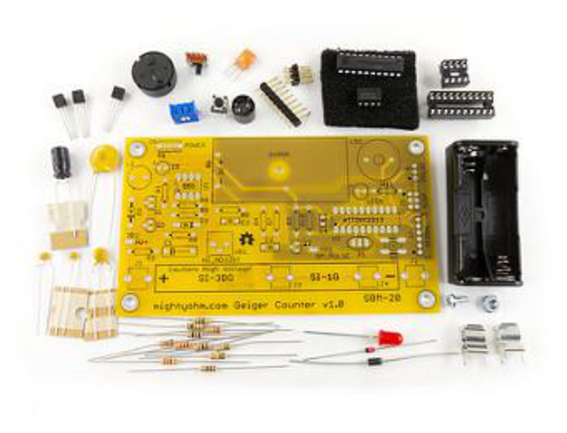
\includegraphics[width=0.45\textwidth]{./images/gconkit.eps}
	      \label{fig:gconkit_before}
	    }
            \hfill
  \subbottom[MightyOhm Geiger Conuter Kit]
	    {
	      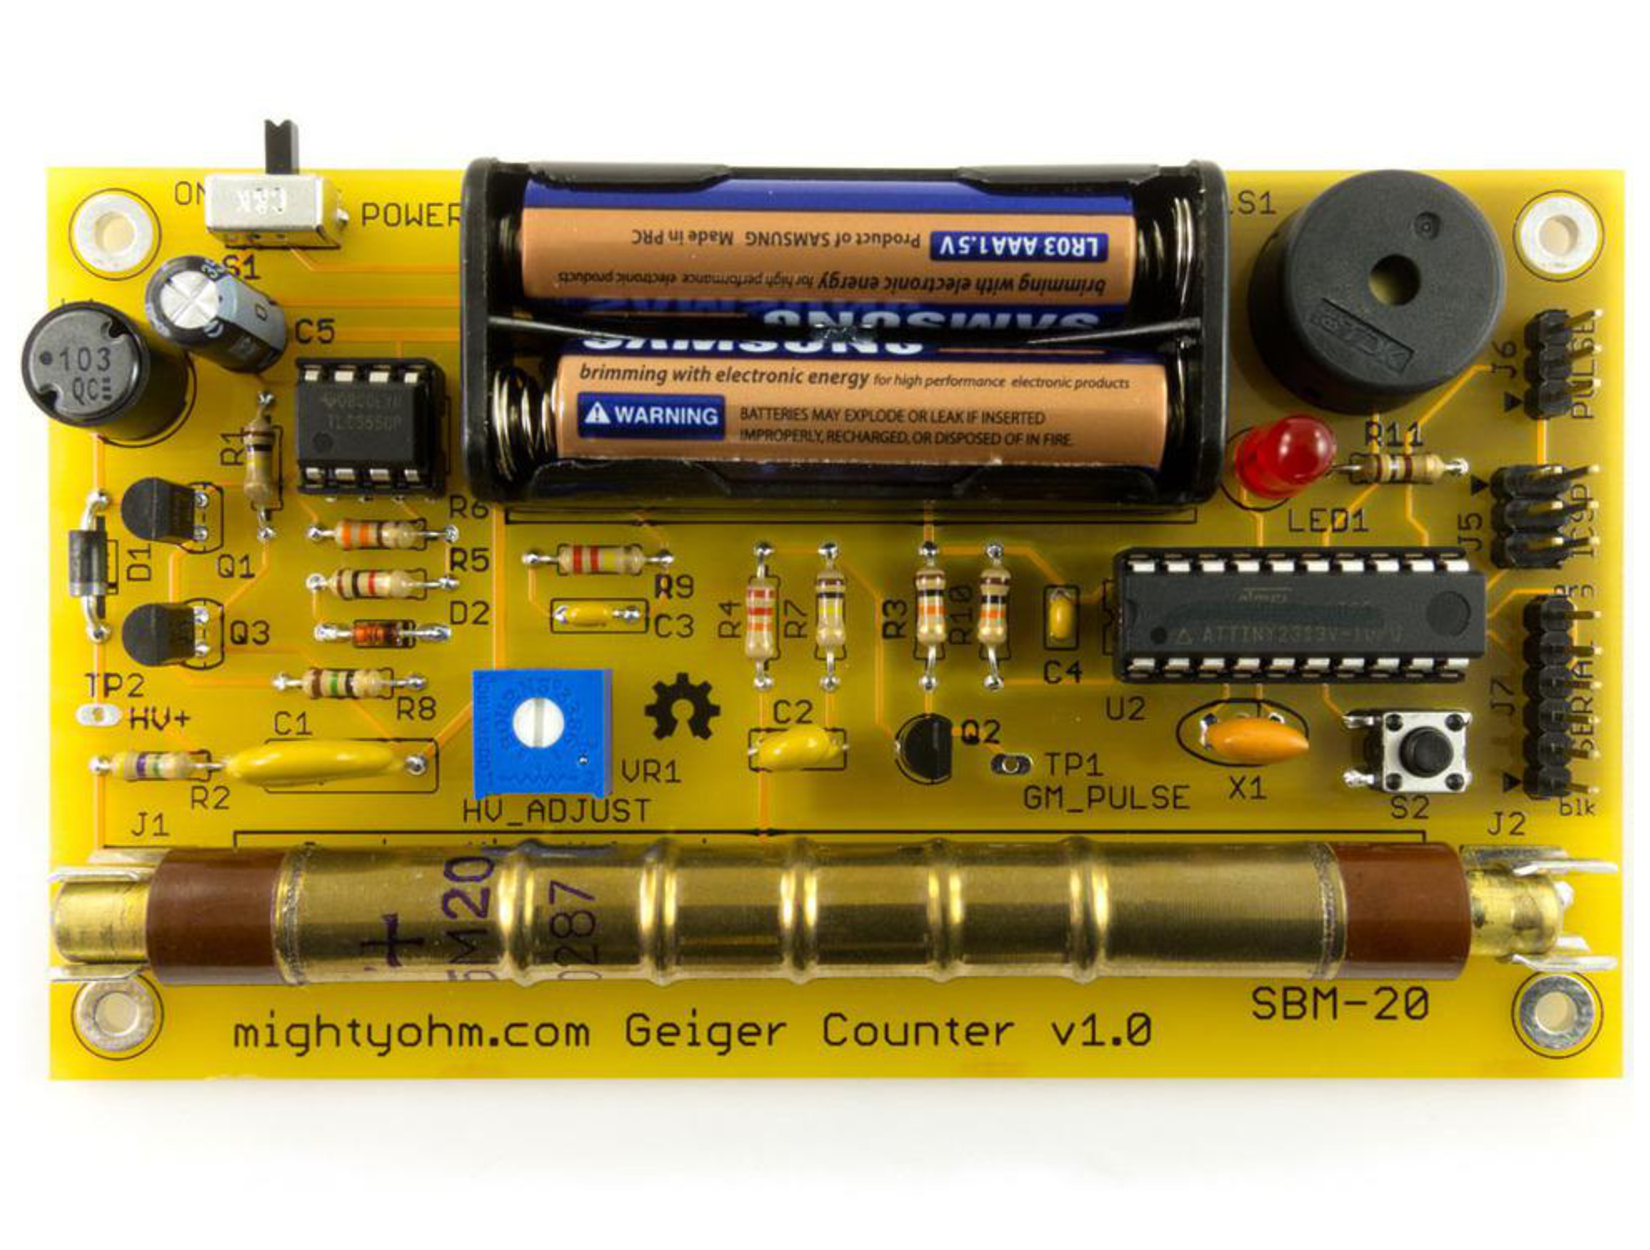
\includegraphics[width=0.45\textwidth]{./images/gconkit_done.eps}
	      \label{fig:gconkit_done}
	    }
  \caption
      {
        MightyOhm Geiger Conuter Kit
      }
 \label{fig:gconkit}
\end{figure}

\vspace{4cm}

\chapter{Raspberry Pi를 이용한 Geiger Counter Kit 구동}

\section{minicom을 이용한 Serial 통신}

\begin{enumerate}
\item 소프트웨어 설치\\
본 문서는 Serial 통신 확인을 위해 minicom을 사용한다. 따라서 Raspberry Pi에 minicom을 설치한다.

\begin{lstlisting}[style=termstyle]
pi@raspberrypi ~ $ sudo aptitude install minicom
\end{lstlisting}

\item Pin Connection\\
Geiger Counter는 시리얼 통신을 위한 6개의 pin이 있으며, 각 pin은 표 \ref{table:pinconnection}과 같이 Raspberry Pi의 GPIO pin과 연결된다. 또한, 기존의 Geiger Conunter Kit은 2개의 AAA배터리를 사용하지만 Raspberry Pi를 이용한 전원 공급을 위해 그림 \ref{fig:drive_gconpi}와 같이 배터리 홀더가 아닌 pin header를 사용해 Raspberry Pi의 GPIO를 통해 전원을 공급한다.

\begin{figure}[h!]
  \centering
  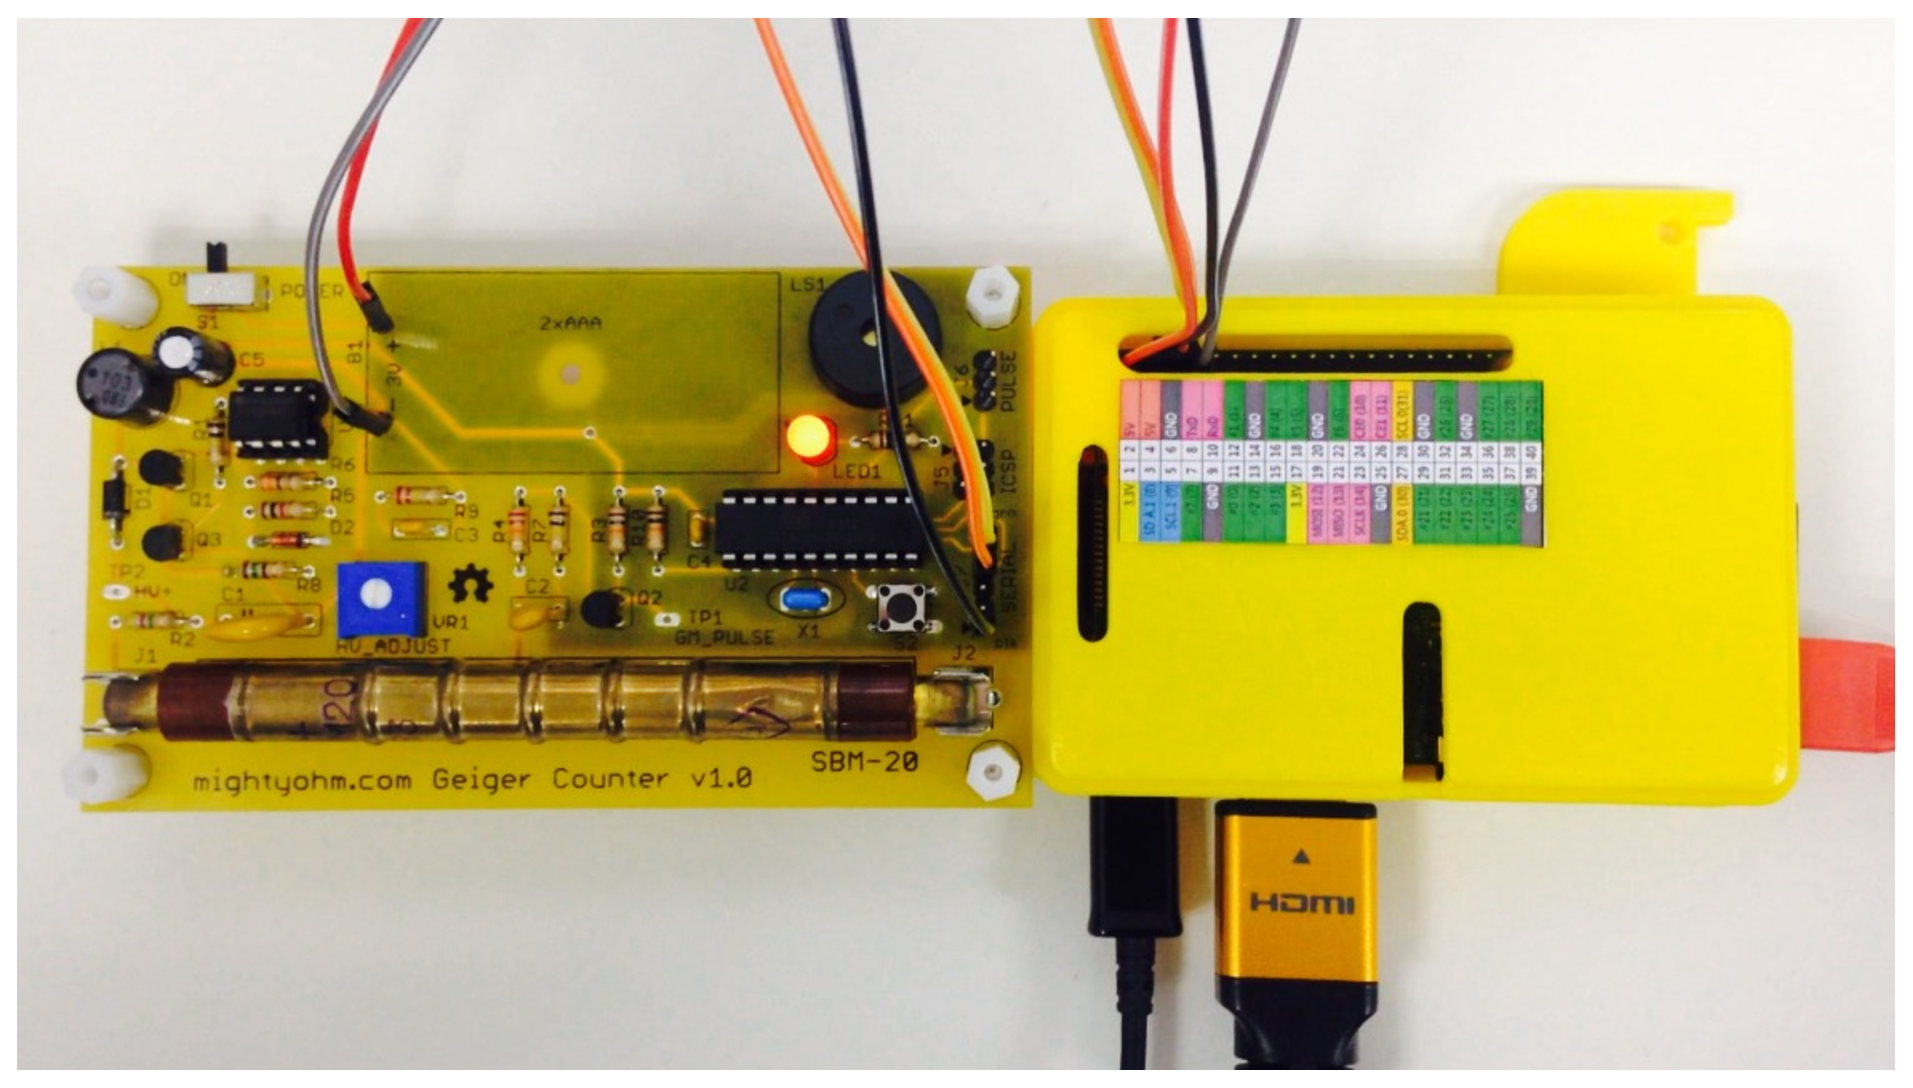
\includegraphics[width=0.8\textwidth]{./images/geiger+rpi.eps}
  \caption{Raspberry Pi로 구동한 Geiger Counter Kit}
  \label{fig:drive_gconpi}   
\end{figure}


\begin{table}[h!]
\begin{center}
\begin{tabular}{lcccc} \hline
&& Serial Connection &&\\
\multicolumn{2}{c}{Geiger Conunter Kit} & & \multicolumn{2}{c}{Raspberry Pi}\\
\cmidrule(r){1-2}\cmidrule(lr){4-5}  
Pin Num (color) & Name & & Pin Num & Name \\ 
1 (Black) & GND & - - - - - - - - - - - - - - - & 6 & GND  \\
2 (Brown) & GND & & & \\
3 (Red) & & & & \\ 
4 (Orange) & RxD  & - - - - - - - - - - - - - - - & 8 & TxD \\ 
5 (Yellow) & TxD  & - - - - - - - - - - - - - - - & 10 & RxD \\
6 (Green) & & & & \\ \hline
&&&&\\ \hline\hline
&& Power Connection &&\\
\multicolumn{2}{c}{Geiger Conunter Kit} & & \multicolumn{2}{c}{Raspberry Pi}\\
\cmidrule(r){1-2}\cmidrule(lr){4-5}  
\multicolumn{2}{c}{Name} & & Pin Num & Name \\ 
\multicolumn{2}{c}{Battery +} & - - - - - - - - - - - - - - - & 1 & 3.3V \\ 
\multicolumn{2}{c}{Battery -} & - - - - - - - - - - - - - - - & 9 & GND \\ \hline
\end{tabular}
\caption{Pin 연결 구성도}
  \label{table:pinconnection} 
\end{center}
\end{table} 

\clearpage

\item Serial 통신 설정\\
Serial 통신을 위한 설정은 다음과 같다.
    {\scriptsize
\begin{itemize}
\item Baud: 9600
\item Data Bits: 8
\item Stop Bits: 1
\item Parity: None
\item Hardware Flow Control: None
\item Software Flow Control: Off (nothing selected)
\end{itemize}
}

아래의 명령어 중 하나를 사용해 Serial 통신을 시작한다. 
\begin{lstlisting}[style=termstyle]
pi@raspberrypi ~ $ sudo minicom -b 9600 -o -D /dev/ttyAMA0
\end{lstlisting}


\begin{lstlisting}[style=termstyle]
pi@raspberrypi ~ $ sudo minicom -s
    +-----------------------------------------------------------------------+
    | A -    Serial Device      : /dev/ttyAMA0                              |
    | B - Lockfile Location     : /var/lock                                 |
    | C -   Callin Program      :                                           |
    | D -  Callout Program      :                                           |
    | E -    Bps/Par/Bits       : 9600 8N1                                  |
    | F - Hardware Flow Control : No                                        |
    | G - Software Flow Control : No                                        |
    |                                                                       |
    |    Change which setting?                                              |
    +-----------------------------------------------------------------------+
\end{lstlisting}

\item Geiger Counter Kit의 전원 ON\\
전원을 키면 Welcome 메세지와 함께 데이터를 확인할 수 있다\citep{datalogging}.
\begin{lstlisting}[style=termstyle]
Welcome to minicom 2.6.1

OPTIONS: I18n 
Compiled on Apr 28 2012, 19:24:31.
Port /dev/ttyAMA0

Press CTRL-A Z for help on special keys

mightyohm.com Geiger Counter 1.00
http://mightyohm.com/geiger

CPS, 1, CPM, 1, uSv/hr, 0.00, SLOW
CPS, 0, CPM, 1, uSv/hr, 0.00, SLOW

\end{lstlisting}
\end{enumerate}

\chapter{EPICS IOC}
\citep{gconpi}




\clearpage
\bibliographystyle{unsrtnat}
\bibliography{./refs}

\end{document}
